\documentclass[12pt]{article}

\usepackage{times}
\usepackage[final]{graphicx}
\usepackage{hyperref}
\usepackage{color}
\usepackage{verbatim}

\setlength{\topmargin}{-0.5in}
\setlength{\oddsidemargin}{0in}
\setlength{\evensidemargin}{0in}
\setlength{\textwidth}{6.5in}
\setlength{\textheight}{9.0in}

\begin{document}

\centerline{\bf \Large CS295/CS395/CSYS395: \href{CS295\_395\_Syllabus.pdf}{\underline{Evolutionary Robotics}}}

\vspace{0.5cm}

\centerline{\bf \large Programming Assignment 6 of 10}
\vspace{0.25cm} \centerline{\color{red}DRAFT: Port from ODE to Bullet by Shane Celis \color{black}}

\vspace{0.5cm}

\centerline{\large Assigned: Friday, October 7, 2011}

\vspace{0.5cm}

\centerline{\large Due: Friday, October 14, 2011 by midnight}

\vspace{0.5cm}

\noindent \color{red}CHANGES: Added tasks of converting from a world coordinate system to a local coordinate system, which bullet uses to make joints.  Added a task to create a command to advance the simulation one time-step.\color{black}

\noindent \textbf{Description:} In this week's assignment you will be adding eight joints to connect together the nine body parts comprising the robot (Fig. \ref{Fig1}). You will accomplish this in the same way as for adding bodies to Bullet: add one joint, compile and run the application so that you can see the effect of the addition on the simulation, only then add a second joint, and so on.

\begin{enumerate}

\item Back up Assignment\_5 on a flash drive or another computer so that you can always return to your completed fifth assignment.

\item Copy directory Assignment\_5, which contains your submitted document and the entire Bullet folder. Rename the new directory Assignment\_6.

\item In the top of \verb|RagdollDemo.h|, find the variables we added last assignment
\begin{verbatim}
    btRigidBody*      body[9]; // one main body, 4x2 leg segments
    btCollisionShape* geom[9];
    bool pause;
\end{verbatim}
and add the following variables
\begin{verbatim}
    btHingeConstraint* joints[8];
    bool oneStep;
\end{verbatim}

\item Before creating joints, we need to grapple to different
  coordinate systems.  Up till now the only coordinate systems
  discussed have been the world coordinate system.  However, each body
  has its own coordinate system where the center of mass is its origin
  (0,0,0) and may rotate.  Run the simulation, hit 'w' to turn on the
  wireframe mode.  You will see red, green, and blue axes markers that
  shows a body's local coordinate system.

\item Write a function in \verb|RagdollDemo.h| with this signature:
  \\\verb|btVector3 PointWorldToLocal(int bodyIndex, btVector3 point)|.
  Look up documentation on the method \verb|getCenterOfMassTransform|
  and the class \verb|btTransform|.  Test that it works by printing
  out the local coordinate of the box's center of mass:
  \\\verb|PointWorldToLocal(0, btVector3(0.,1.,0.))|.  The result
  should be (0,0,0).

\item Write a variant of the preceding function that converts an axis
  vector, or direction vector, from the world coordinate system to a
  body's local coordinate system in \verb|RagdollDemo.h| with this
  signature:
  \\\verb|btVector3 AxisWorldToLocal(int bodyIndex, btVector3 point)|.
  If your main body has not been rotated, you can test that it works
  by printing out the result of
  \verb|AxisWorldToLocal(0, btVector3(0.,1.,0.))|.  The result should
  be (0,1,0).


\item Now create a function \texttt{CreateHinge(int index,...)} in
  \verb|RagdollDemo.h| that will create a joint. You will need to pass
  this function a number of parameters: you need to tell it which two
  bodies to attach together; where the joint's fulcrum should be; and
  the axis of the joint. If you are unfamiliar with these concepts,
  refer to the Lecture 6 on physical simulation.

\item Inside the \verb|CreateHinge| function you will use these
  parameters to create a hinge joint (\verb|new btHingeConstraint()|).
\begin{verbatim}
btHingeConstraint(btRigidBody& rbA,    btRigidBody& rbB, 
                  btVector3& pivotInA, btVector3& pivotInB, 
                  btVector3& axisInA,  btVector3& axisInB)
\end{verbatim}

Note that the vector arguments to this constructor are given in the
local coordinate systems of bodies A and B.  At the end of the
function, you'll want to add the joint to the simulation using the
following line:
\begin{verbatim}
      m_dynamicsWorld->addConstraint(joints[index], true);
\end{verbatim}

\item Create another function \texttt{DestroyHinge(int index)} that removes the joint from the simulation.

\item Add a line \texttt{CreateHinge(0,...);} that creates the first joint, which attaches the right lower leg to the right upper leg (Fig. \ref{Fig1}a). This line should be placed just after all of the bodies have been created.

\item Add \texttt{DestroyHinge(0);} to the \verb|exitPhysics| method.  Recompile and rerun until there are no errors and you can restart the simulation by hitting the space key with no errors.

\item Compile and run the simulation in paused mode. You should see that, as the right upper leg falls, it is stays connected to the right lower leg at the `knee'. You should see something like that of Fig. \ref{Fig1}a. However, this may happen to fast to capture the screen, so we'll need to add an ability do one step at a time.

\item We want to add the ability to pause the simulation and with one key press advance the simulation only one time step.  In the method \verb|clientMoveAndDisplay|, edit the call to \verb|stepSimulation| so that it will run one step if it is paused and the variable \verb|oneStep| is true.  \verb|oneStep| should then be set to false.  Recompile and rerun until there are no errors.

\item Edit the \verb|keyboardCallback| method so that when the key 'o' is pressed \verb|oneStep| is set to true.  Recompile and rerun until you can pause the simulation and hitting 'o' advances the simulation one time step.

\item Compile and run the simulation in paused mode.  Press 'o' to repeatedly step through the simulation.  You should see that, as the right upper leg falls, it stays connected to the right lower leg at the 'knee'.  You should be able to capture the screen with something like Fig. \ref{Fig1}a. Store this image in your document.

\item Now add the second joint that connects the left upper leg to the left lower leg, recompile and rerun.

\item Add the third joint that connects the front (into the screen) upper leg to the front lower leg, recompile and rerun.

\item Add the fourth joint that connects the back (toward the viewer) upper leg to the back lower leg, recompile and rerun. This should now produces an image like that in Fig. \ref{Fig1}b. Screen capture and store in your document.

\item Using the same procedure, add the fifth joint that connects the right upper leg to the main body. Recompile, rerun and step through the simulation to get an image like that in Fig. \ref{Fig1}c. Screen capture and copy into your document.

\item Now iteratively add the sixth, seventh and eighth joint connect the remaining three legs to the main body. The robot should now `sit down', and its legs should flatten out, producing an image as in Fig. \ref{Fig1}d.

\item We now need to constrain the range of motion of each joint. For simplicity, we will set each joint to only rotate through $[-45^o,45^o]$. To do this, you will need to add this line to \texttt{CreateHinge(...)}: 

  \begin{verbatim}
    joints[index]->setLimit(-45.*3.14159/180., 45.*3.14159/180.);
  \end{verbatim}
  What is the \texttt{x*(3.14159./180.)} for?

\item Now when you recompile and rerun the simulation you should obtain an image as in Fig. \ref{Fig1}e. Screen capture and copy into your document, and submit your document.

\end{enumerate}

\begin{figure}[!t]
\centerline{
a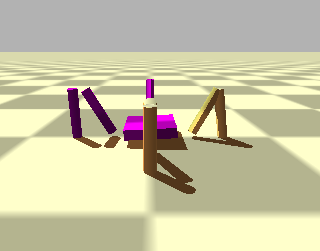
\includegraphics[width=0.25\textwidth]{Fig1a}
b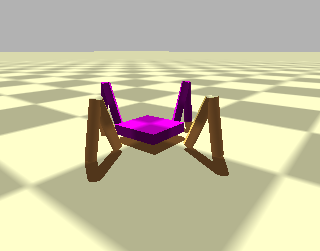
\includegraphics[width=0.25\textwidth]{Fig1b}
c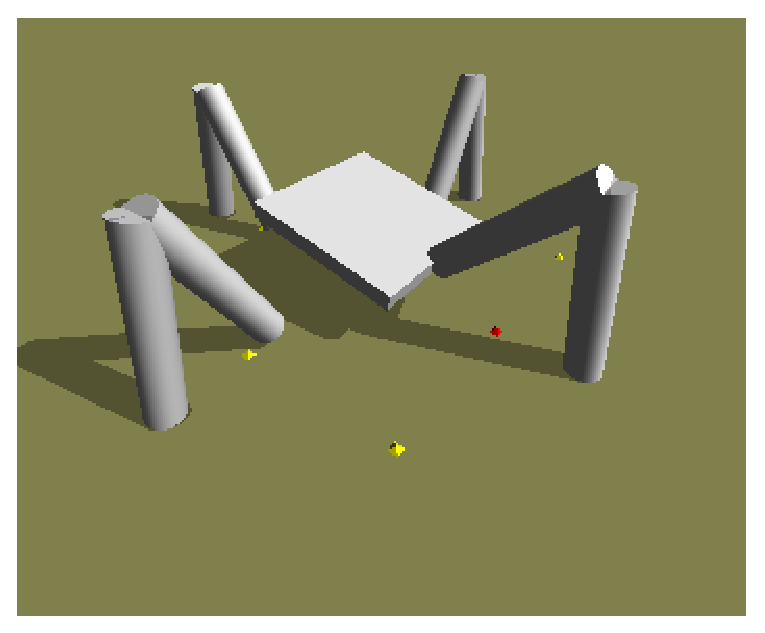
\includegraphics[width=0.25\textwidth]{Fig1c}}
\centerline{
d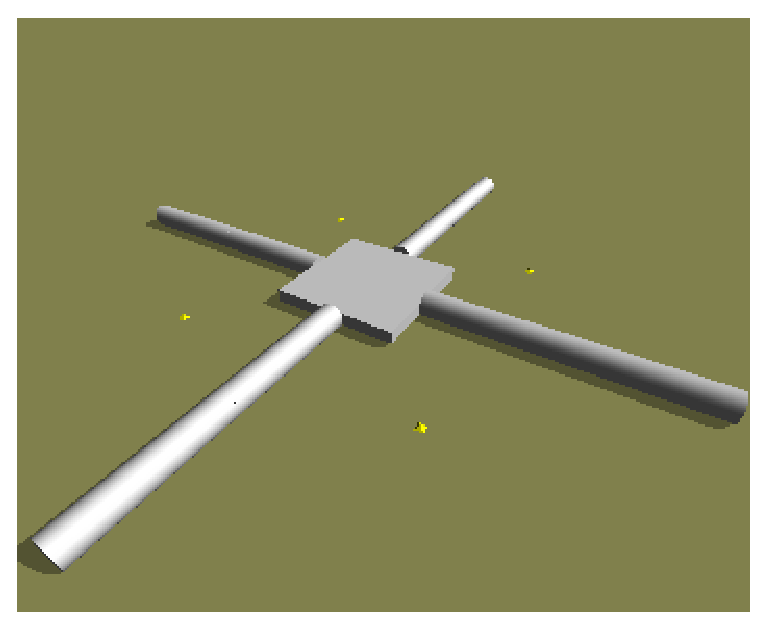
\includegraphics[width=0.25\textwidth]{Fig1d}
e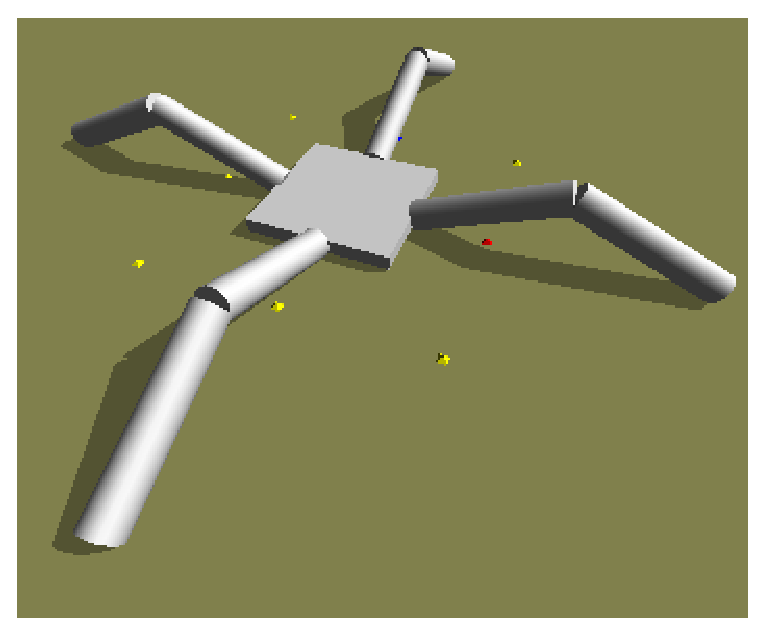
\includegraphics[width=0.25\textwidth]{Fig1e}}
\caption{Incremental addition of joints to the quadrupedal robot.}
\label{Fig1}
\end{figure}

\end{document} 
